\subsection{Феномен тесного мира}

Для того чтобы понять, каким должен быть граф для 
оптимальной работы нашего алгоритма, я предлагаю обратиться
к структурам, которые возникают само собой в приро\-де, 
к графам, которые формирует общество.

\subsubsection{Теория 6 рукопожатий}

Венгерский писатель Karinthy Frigyes Ernő в 1928г в рассказе 
"Звенья цепи" впервые сформулировал данную проблему. Согласно ей, 
любые два человека на планете связаны через 5-6 общих знакомых.

Рассуждая над этой проблемой, Stanley Milgram - американский 
социальный психолог и педагог в своей статье "The Small World Problem" \cite{Milgram}
описал проведённый им экспе\-римент: 
Он выдал 300 писем жителям из разных городов и попросил доставить 
их одному человеку из Бостона (США). Важным условиям было то, что
люди могли передавать письма только своим знакомым, которые по их
мнению могли знать целовека-цель.
По результатам ис\-следования, даже не смотря на то, что до места назначения
дошли далеко не все письма, те, которым это удалось, прошли в среднем через цепь из
5-6 человек. 

Данные наблюдения кажутся очень полезными для нас. Ведь если нам
удастся вос\-создать граф, который с хорошей точностью моделируют
общественные сети, мы сможем из любой вершины графа добираться до 
цели за сравнимо малое число посредников. Причём для этого нам даже 
не придётся использовать сложные алгоритмы поиска. Вспом\-ним эксперимент
Милгрема, в нём каждый человек не пытался искать оптимальный путь
от него до цели, он лишь отправлял письма тем знакомым, которые казались
ближе к месту назначения. Формально - это простой жадный поиск, который
в эксперименте Милгрема прошёлся всего лишь по 5-6 промежуточным значениям
и, что не мало важно, достиг цели.

% Однако, при попытке смоделировать данное поведение на компьютере, даже
% на небольшой выборке значений, это не сработает. Если мы построим
% граф, который будет состоять из кластеров вершин (вершины, соеденины
% ребром только в случае, если они находятся рядом), его диаметр будет
% всё равно очень большим. То есть, чтобы добраться от одной вершины
% к другой, понадобиться много посредников

\subsubsection{Случайные графы Erdős–Rényi}
Попробуем предположить, что общественные сети можно
представить, как случайный граф $G(n, p) = \{V, E\}$ состоящий из $n$ вершин, с
вероятностью проведения ребра p. Логично предположить, что $np = const = \lambda$.
Можно объяснить это так: структура графа не должна зависить от кол-ва
вершин в нём. Он всегда должен выглядеть примерно одинаково ($deg(v) \approx const$). Ну или ещё
одно описание: кол-во моих друзей не увеличится, если население планеты 
увеличится в несколько раз. Обоснуем это формально:
\begin{equation}
    P(deg(v) = k) = \binom{n}{k}p^k(1-p)^{1-k}
    \Rightarrow deg(v) \sim Bin(p)
\end{equation}
Так как $np = const = \lambda : \mathbb{E}[deg(v)] = np = \lambda$

Так мы описали граф, изучением которого занимались
два великих Венгерских мате\-матика Paul Erdős и Alfréd Rényi. (Причём $\lambda$ обычно
выбирается много меньше чем $n$, ведь наш круг общения никчёмно мал по сравнению с 8 млрд. людей на
планете) 

Разультаты, к которым пршли данные математики, показали, что случайные графы имеют 
сравнительно малый средний диаметр $d(G)$. Где
\begin{equation}
    d(G) = \frac{1}{|V|}\sum_{u, v \in V}d(u, v)
\end{equation}
\begin{equation}
    d(u, v) = \min_{k \in \mathbb{R}}\{\exists a_i, \ i = \overline{1k}  : a_1 = u, a_{k + 1} = v, (a_i, a_{i + 1}) \in E\}
\end{equation}
Казалось бы, малый диаметр - всё, что нам нужно. И это было бы так, если бы мы не 
использовали жадный алгоритм для поиска. Случайные рёбра в графе помогают 
нам легко и быстро приблизиться к месту назначения, однако отсутствие локальных
рёбер приводит к большому кол-ву локальных минимумов, что ведёт за собой большую
погрешность в полученном результате, пример:

\begin{figure}[H]
\centering
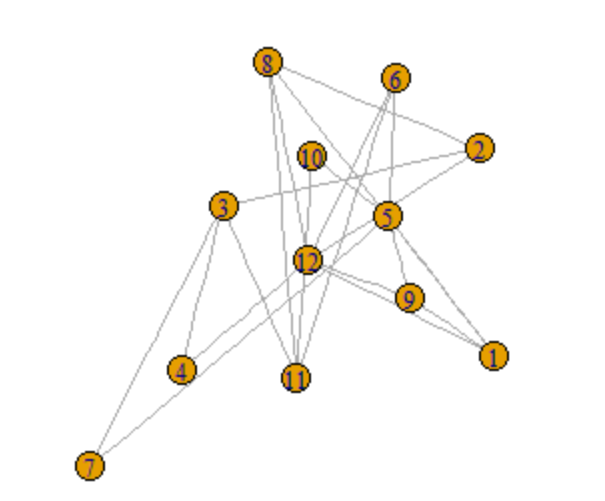
\includegraphics[scale=0.3]{./pictures/random_graph.png}
\caption{Случайный граф} \label{random_graph}
\end{figure}

Взглянув на рисунок \ref{random_graph}, можно заметить, что если мы хотим добраться до вершины 3,
используя жадный поиск, то это нам удастся только из непосредственных соседей вершины номер 3.
Это говорит о том, что такой граф хорош в навигации на больших масштабах, но плох при локальном
поиске. Это не состыкуется с теорией 6 рукопожатий

Ошибка в наших рассуждениях была в том, что мы предположили, что связи между людьми абсолютно
случайны, но ведь это не так. Милгрэм, описывая результаты своего эксперимента, делал акцент
на то, что общественные графы состоят из кластеров. Это можно описать так: Вероятность знакомства
с человеком тем больше, чем мы ближе; А также, вероятность, того, что люди дружат прямо пропорциональна
кол-ву их общих друзей. Наличие данной концепции образовало бы больше локальных рёбер, что решило бы
проблему локальных минимумов. Формально это можно описать разными способами, например, через коэффицент кластеризации вершины:
\begin{equation*}
    cc(v) = \frac{\#\{(x, y) \in E, \ x, y \in V: (x, v), (y, v) \in E\}}
    {\#\{(x, y), \ x, y \in V: (x, v), (y, v) \in E\}}
\end{equation*}
По аналогии коэффицент кластеризации графа:
\begin{equation*}
    cc(G) = \frac{1}{|V|}\sum_{v \in V}cc(v)
\end{equation*}
Чем он больше, тем сильнее кластеризован наш граф. 

\subsubsection{Тесные графы}
    В рассуждениях выше мы пришли к выводам, что графы в реальном мире обладают
двумя основными свойствами: малым диаметром и большим коэффицентом кластери\-зации.
В 1998г, наблюдая за реальными сетями, к тем же самым выводам пришли два американских 
математика: Дункан Уоттс и Стивен Строгац. Они выделили такие графы в отдельную группу
"Тесные графы". формально их можно записать так:
\begin{equation*}
    \bigg(G(U, V) - \text{Тесный граф}\bigg) \Leftrightarrow
    \begin{cases}
        d(G) \approx 0 \\
        cc(G) \approx 1
    \end{cases}
\end{equation*}

В практической части, будет показано, что $cc(G) \rightarrow 0$ с ростом n, где G - случайный граф
по модели Erdos-Renye

% Давайте докажем, что в случайный граф не подходит под это определение.
% Докажема, что коэффицент кластеризации стремится к 0 с ростом n: \\
% Для начала посчитаем $\mathbb{E}[cc(v)]$. Обозначим $N = \binom{deg(v)}{t}, \ t \leq deg(v)$.
% Тогда:
% \begin{equation*}
%     P(N * cc(v) = t) = \binom{N}{t}p^t(1 - p)^{N - t} \Rightarrow N * cc(v) \sim Bin(p) 
% \end{equation*}
% Тогда $\mathbb{E}[N * cc(v)] = Np \Rightarrow \mathbb{E}[cc(v)] = p : \forall N \in \mathbb{N}$
% Заметим, что $cc(v)$  хоть и распределены одинаково, однако не независимы. Я утверждаю, что мы
% этим можем пренебречь, так как $k \ll n$. Данная гипотеза будет обоснована позднее. \\
% Если считать, что $cc(v)$ - i.i.d, то можно использовать УЗБЧ:
% \begin{equation*}
%     cc(G) = \overline{cc(v)} \overset{a.s.}{\rightarrow} 
%     \mathbb{E}[cc(v)] = p = \frac{\lambda}{n} \rightarrow 0, \ n \rightarrow \infty
% \end{equation*}
% Теперь сформулируем гипотезу о независимости:
% \begin{equation*}
%     H_0: cc(u_i) - iid, \ \forall u \in V : k \ll n
% \end{equation*}
% \begin{equation*}
%     H_1: alternative 
% \end{equation*}
Хочется ещё подметить, что тесные графы встречаются очень часто в природе.
Ней\-ронные сети в нашем мозге, карты дорог, пищевые цепочки. Их формирование кажется
вполне логичным. Мозгу необходимо, чтобы сигнал быстро перемещался между нейро\-нами,
для быстрой обработки информации и реакции. Можно утверждать, что другие типы графов
в данных примерах просто не прошли естественный отбор.















